\documentclass[landscape]{article}

\usepackage[utf8]{inputenc}
\usepackage[english]{babel}

\usepackage{amsmath,amsfonts,amssymb}
\usepackage{fullpage}
\usepackage{verbatim}

\usepackage[margin=10mm, top=5mm, bottom=5mm]{geometry}

\usepackage{tikz,pgfplots}

\pgfplotsset{
  width=240mm,height=180mm,
  major grid style={thin,dotted,color=black!50},
  minor grid style={thin,dotted,color=black!50},
  grid,
  every axis/.append style={
    line width=1pt,
    tick style={
      line cap=round,
      thin,
      major tick length=4pt,
      minor tick length=2pt,
    },
  },
  legend cell align=left,
  legend pos=north west,
  compat=1.9
}

%%%%%%%%%%%%%%%%%%%%%%%%%%%%%%%%%%%%%%%%%%%%%%%%%%%%%%%%%%%%%%%%%%%%%%%%%%%%%%%%

\begin{document}

% IMPORT-DATA Results Pivots.txt

\begin{center}

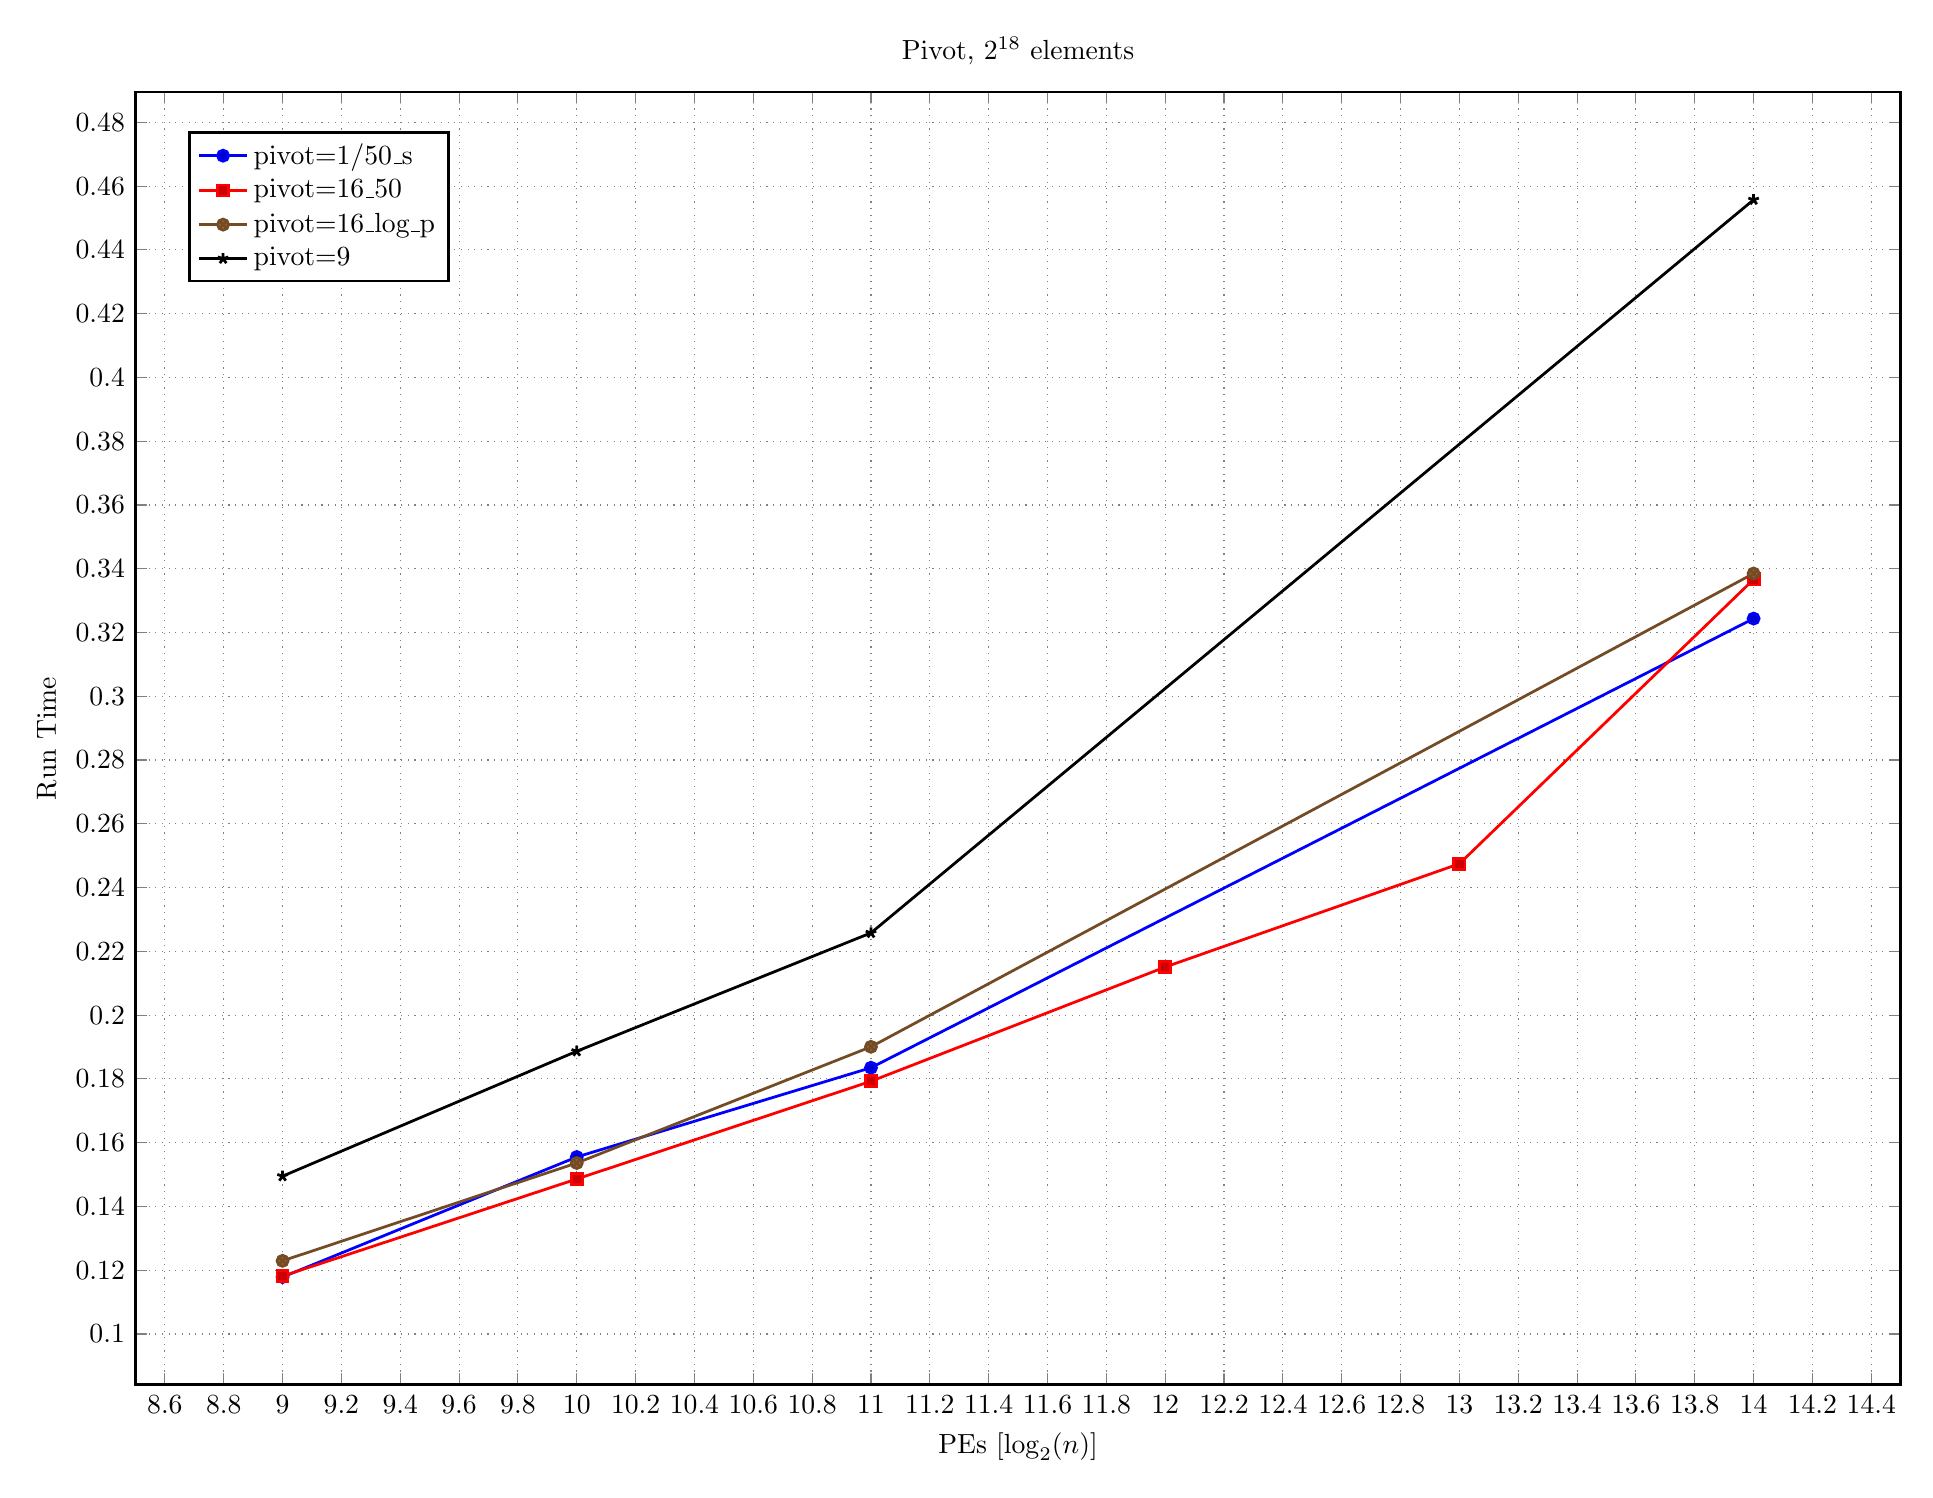
\begin{tikzpicture}
  \begin{axis}[
    title={Pivot, $2^{18}$ elements},
    xlabel={PEs [$\log_2(n)$]},
    ylabel={Run Time},
    ]    

    %% MULTIPLOT(pivot) SELECT LOG(2, size) AS x, MEDIAN(runtime) AS y, MULTIPLOT
    %% FROM Results
    %% WHERE elements=POWER(2,18) AND (pivot="9" OR pivot="16_log_p" OR pivot="1/50_s" OR pivot ="16_50")
    %% GROUP BY MULTIPLOT, x  ORDER BY MULTIPLOT, x
    \addplot coordinates { (9.0,0.117844) (10.0,0.155503) (11.0,0.183499) (14.0,0.324364) };
    \addlegendentry{pivot=1/50\_s};
    \addplot coordinates { (9.0,0.118147) (10.0,0.148598) (11.0,0.179253) (12.0,0.21508) (13.0,0.247469) (14.0,0.336655) };
    \addlegendentry{pivot=16\_50};
    \addplot coordinates { (9.0,0.122932) (10.0,0.153617) (11.0,0.190062) (14.0,0.338498) };
    \addlegendentry{pivot=16\_log\_p};
    \addplot coordinates { (9.0,0.149483) (10.0,0.188666) (11.0,0.225781) (14.0,0.455723) };
    \addlegendentry{pivot=9};

  \end{axis}
\end{tikzpicture}
\newpage

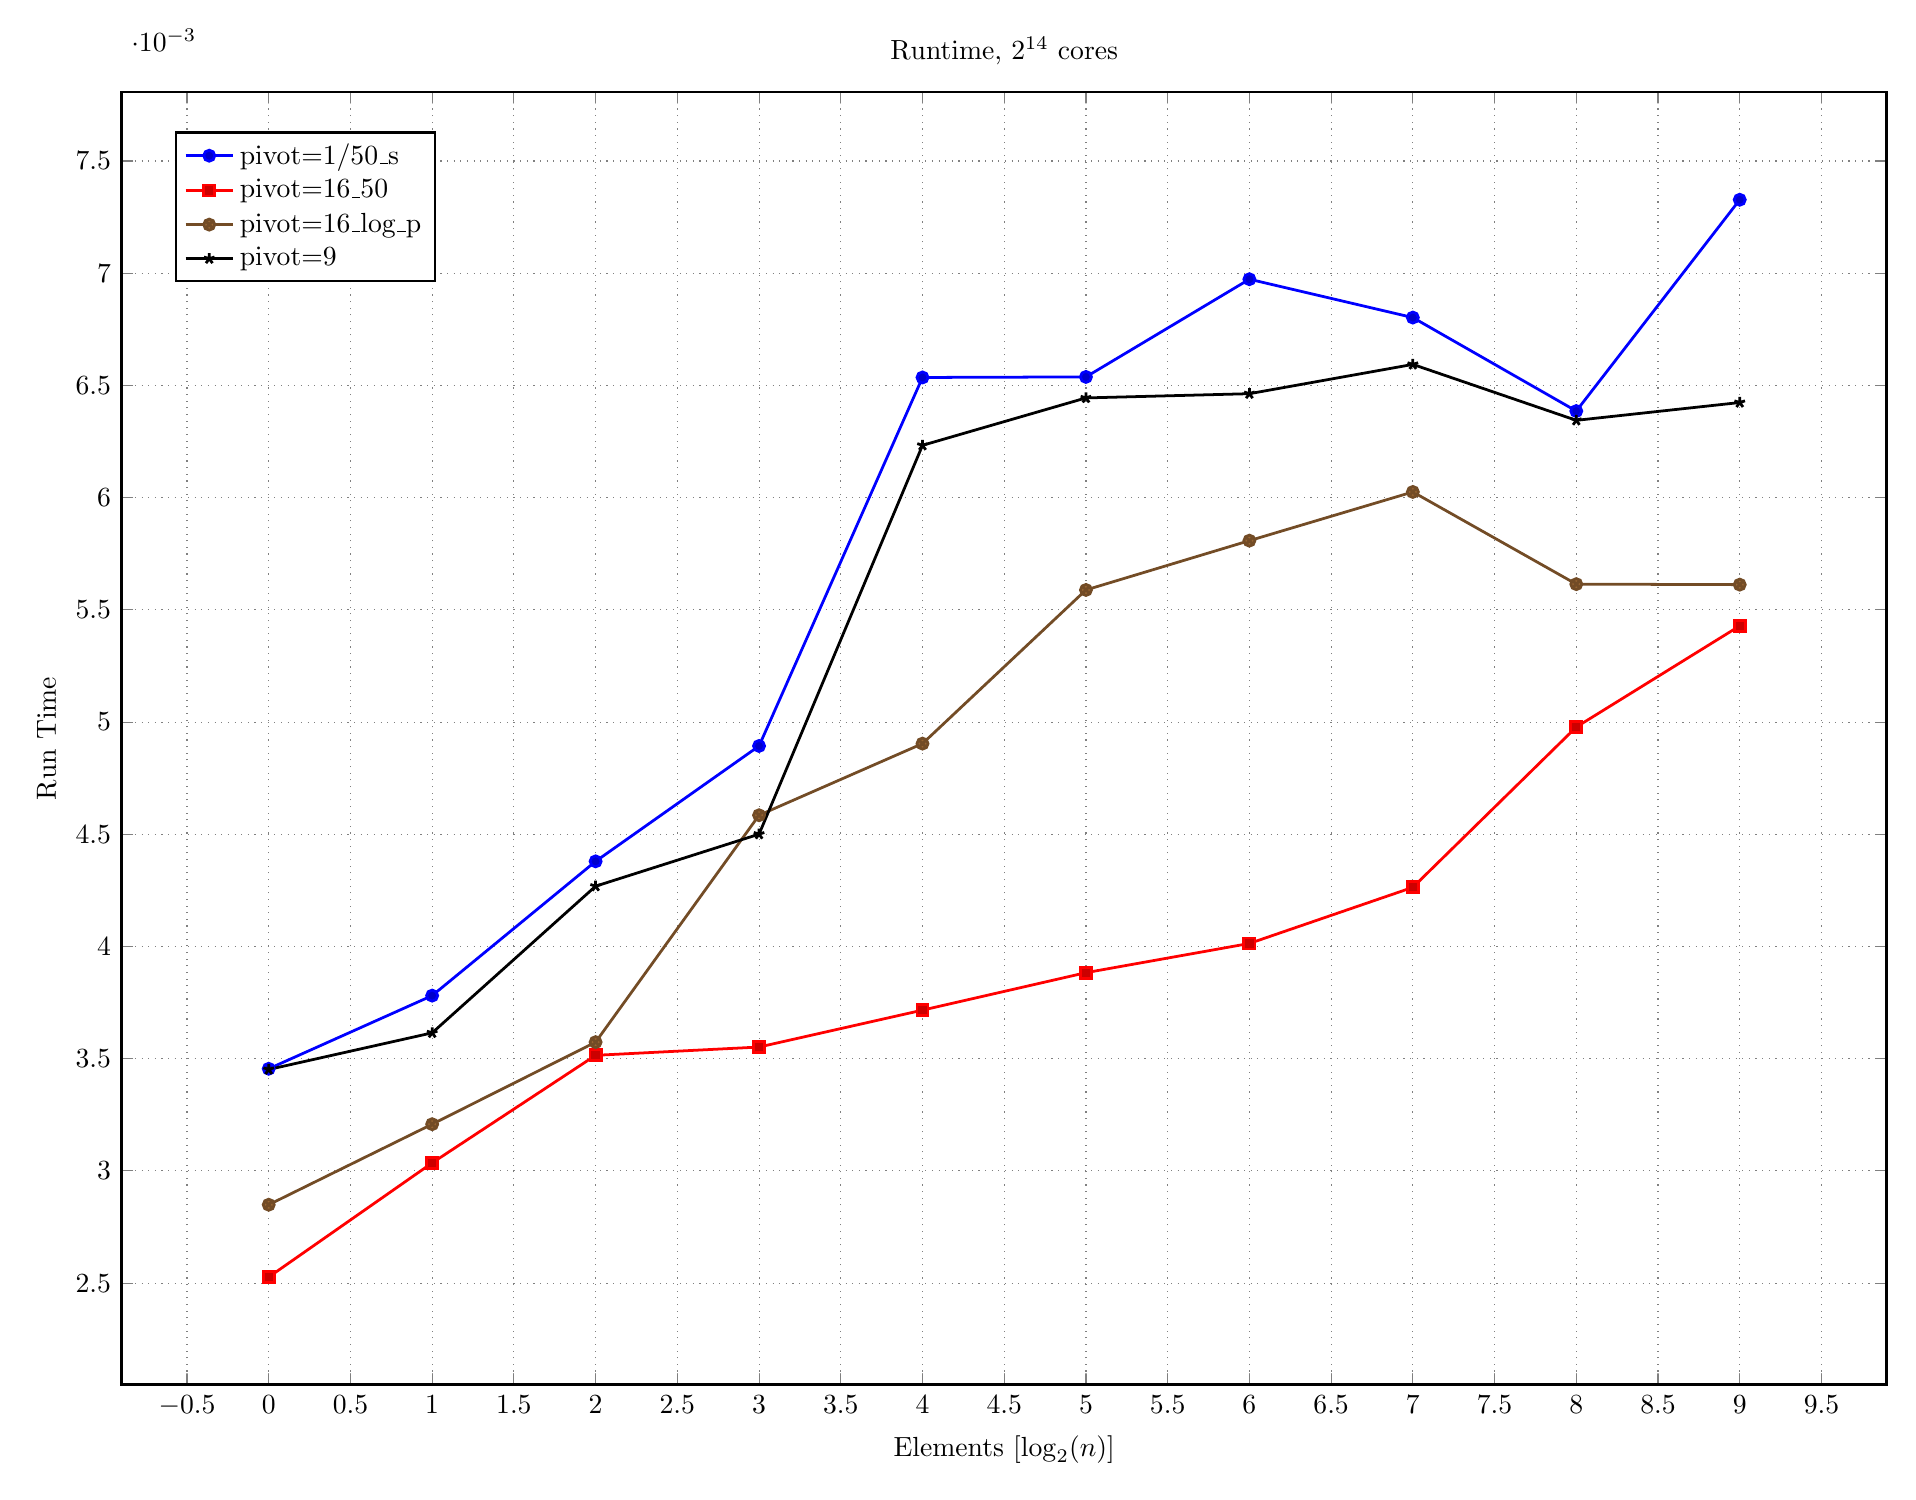
\begin{tikzpicture}
  \begin{axis}[
    title={Runtime, $2^{14}$ cores},
    xlabel={Elements [$\log_2(n)$]},
    ylabel={Run Time},
    ]    

    %% MULTIPLOT(pivot) SELECT LOG(2, elements) AS x, MEDIAN(runtime) AS y, MULTIPLOT
    %% FROM Results 
    %% WHERE size=POWER(2,14) AND x<10 AND (pivot="9" OR pivot="16_log_p" OR pivot="1/50_s" OR pivot ="16_50")
    %% GROUP BY MULTIPLOT, x  ORDER BY MULTIPLOT, x
    \addplot coordinates { (0.0,0.00345508) (1.0,0.00378104) (2.0,0.00437933) (3.0,0.00489346) (4.0,0.00653554) (5.0,0.00653793) (6.0,0.00697331) (7.0,0.00680245) (8.0,0.00638588) (9.0,0.00732747) };
    \addlegendentry{pivot=1/50\_s};
    \addplot coordinates { (0.0,0.00252683) (1.0,0.00303563) (2.0,0.00351498) (3.0,0.00355191) (4.0,0.00371633) (5.0,0.00388328) (6.0,0.00401346) (7.0,0.00426354) (8.0,0.00497777) (9.0,0.00542872) };
    \addlegendentry{pivot=16\_50};
    \addplot coordinates { (0.0,0.00284919) (1.0,0.0032081) (2.0,0.00357376) (3.0,0.00458483) (4.0,0.00490397) (5.0,0.00558869) (6.0,0.00580836) (7.0,0.0060254) (8.0,0.00561461) (9.0,0.00561234) };
    \addlegendentry{pivot=16\_log\_p};
    \addplot coordinates { (0.0,0.00345181) (1.0,0.0036151) (2.0,0.00426861) (3.0,0.00450045) (4.0,0.00623315) (5.0,0.00644438) (6.0,0.00646321) (7.0,0.0065937) (8.0,0.00634449) (9.0,0.00642386) };
    \addlegendentry{pivot=9};

  \end{axis}
\end{tikzpicture}
\newpage

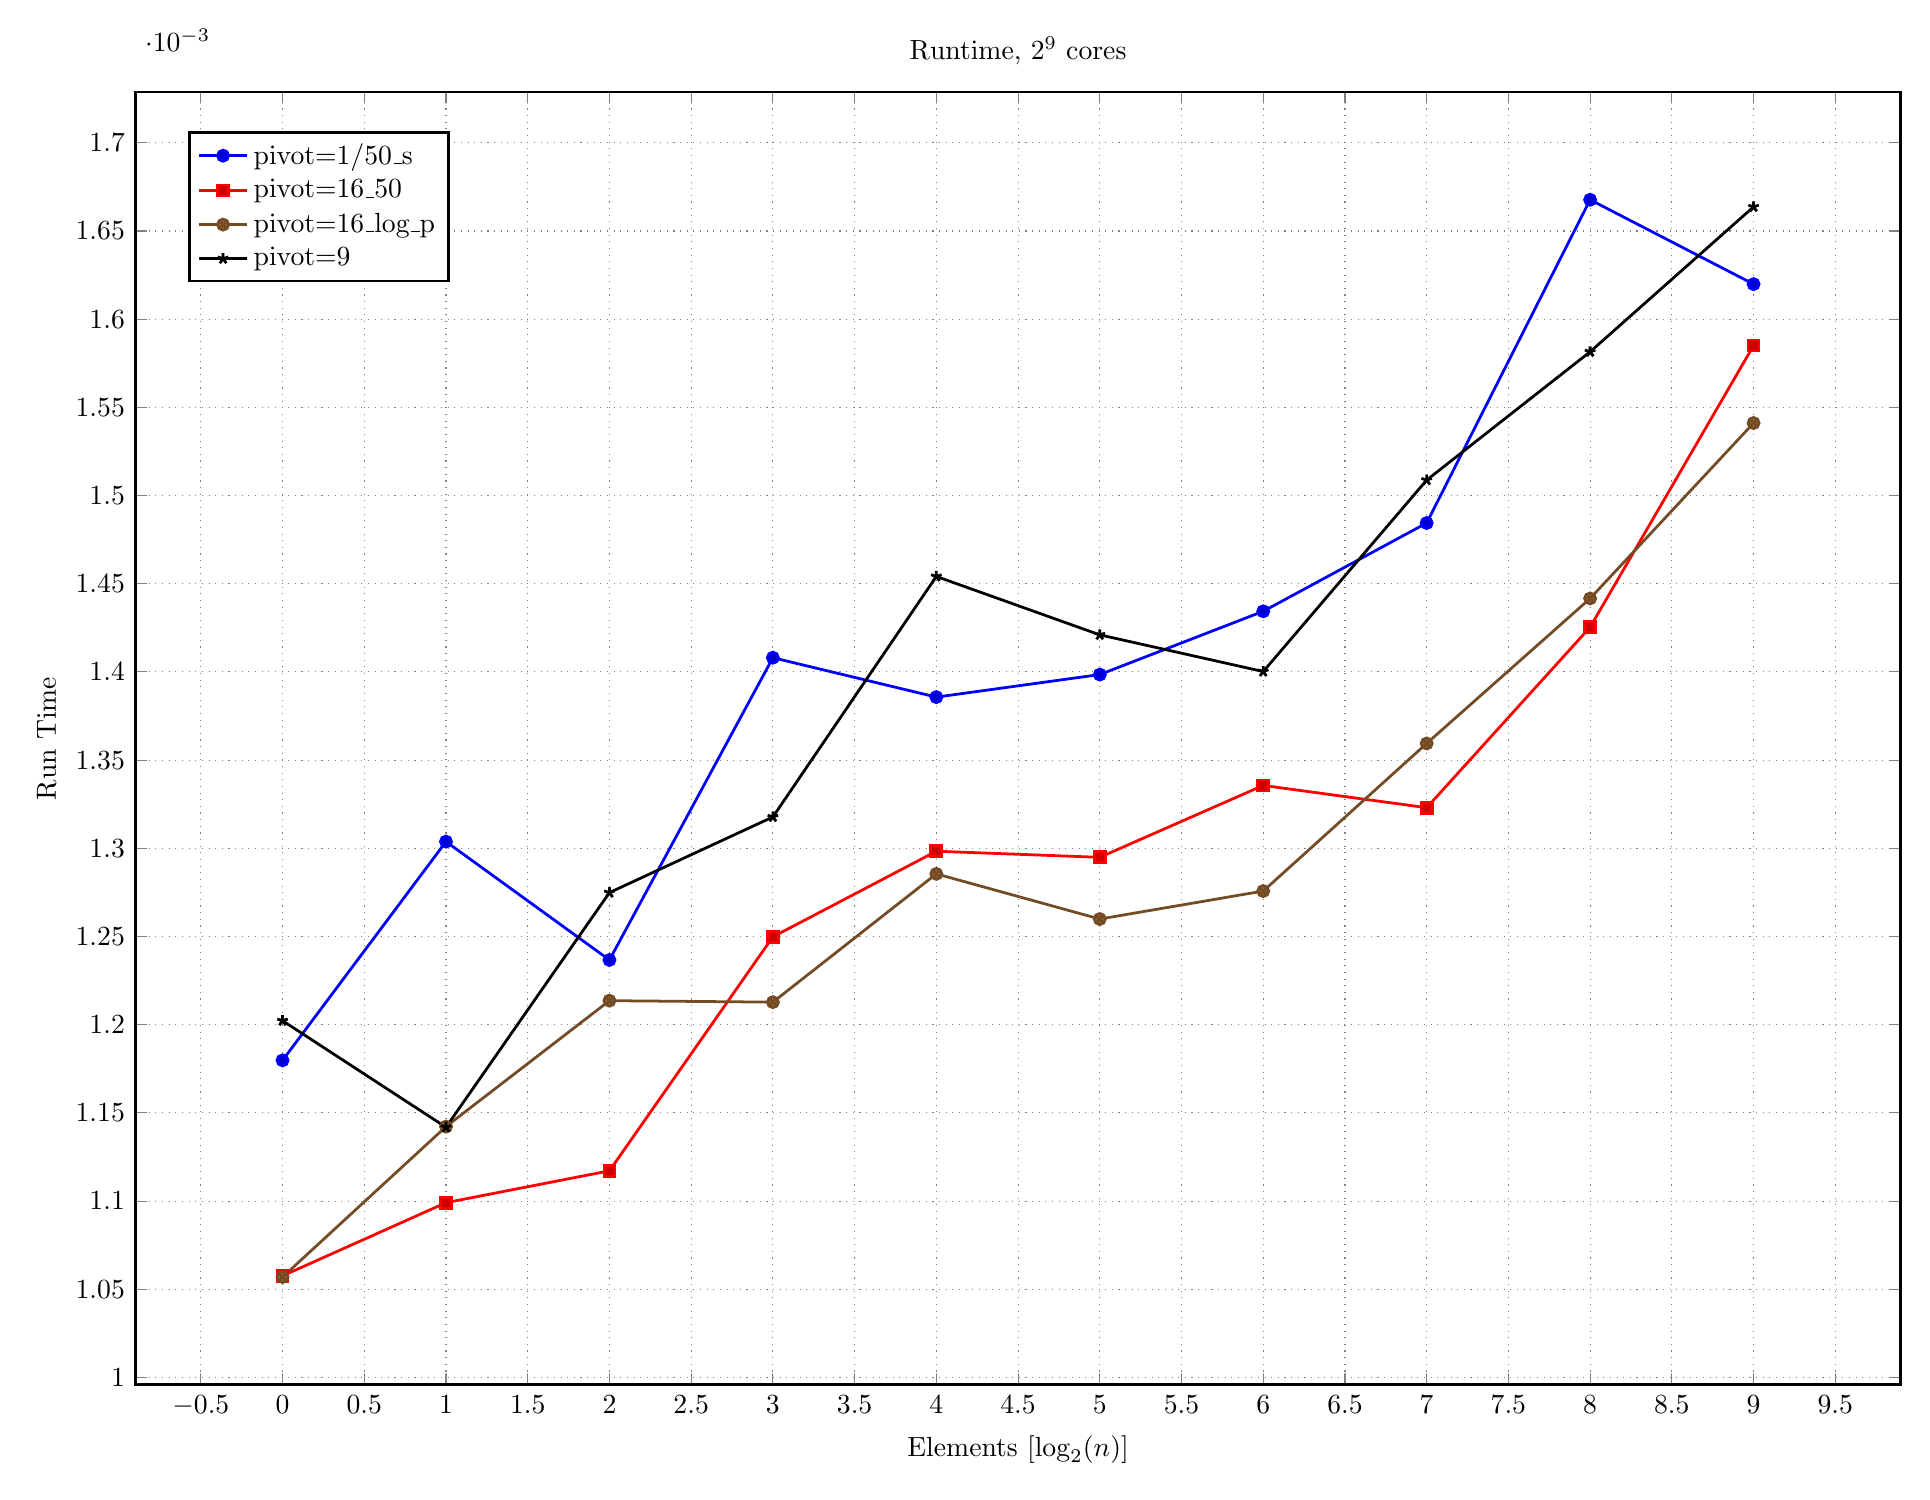
\begin{tikzpicture}
  \begin{axis}[
    title={Runtime, $2^{9}$ cores},
    xlabel={Elements [$\log_2(n)$]},
    ylabel={Run Time},
    ]    

    %% MULTIPLOT(pivot) SELECT LOG(2, elements) AS x, MEDIAN(runtime) AS y, MULTIPLOT
    %% FROM Results 
    %% WHERE size=POWER(2,9) AND x<10 AND (pivot="9" OR pivot="16_log_p" OR pivot="1/50_s" OR pivot ="16_50")
    %% GROUP BY MULTIPLOT, x  ORDER BY MULTIPLOT, x
    \addplot coordinates { (0.0,0.00117978) (1.0,0.0013038) (2.0,0.00123669) (3.0,0.00140807) (4.0,0.00138573) (5.0,0.00139851) (6.0,0.00143439) (7.0,0.00148444) (8.0,0.00166773) (9.0,0.00161988) };
    \addlegendentry{pivot=1/50\_s};
    \addplot coordinates { (0.0,0.0010576) (1.0,0.00109908) (2.0,0.00111715) (3.0,0.00124982) (4.0,0.00129835) (5.0,0.00129489) (6.0,0.00133565) (7.0,0.00132303) (8.0,0.00142537) (9.0,0.00158506) };
    \addlegendentry{pivot=16\_50};
    \addplot coordinates { (0.0,0.00105691) (1.0,0.00114222) (2.0,0.00121361) (3.0,0.00121278) (4.0,0.00128551) (5.0,0.0012599) (6.0,0.00127576) (7.0,0.00135946) (8.0,0.00144167) (9.0,0.00154112) };
    \addlegendentry{pivot=16\_log\_p};
    \addplot coordinates { (0.0,0.00120224) (1.0,0.00114184) (2.0,0.00127489) (3.0,0.00131779) (4.0,0.00145414) (5.0,0.00142103) (6.0,0.00140022) (7.0,0.00150877) (8.0,0.00158152) (9.0,0.00166371) };
    \addlegendentry{pivot=9};

  \end{axis}
\end{tikzpicture}
\newpage

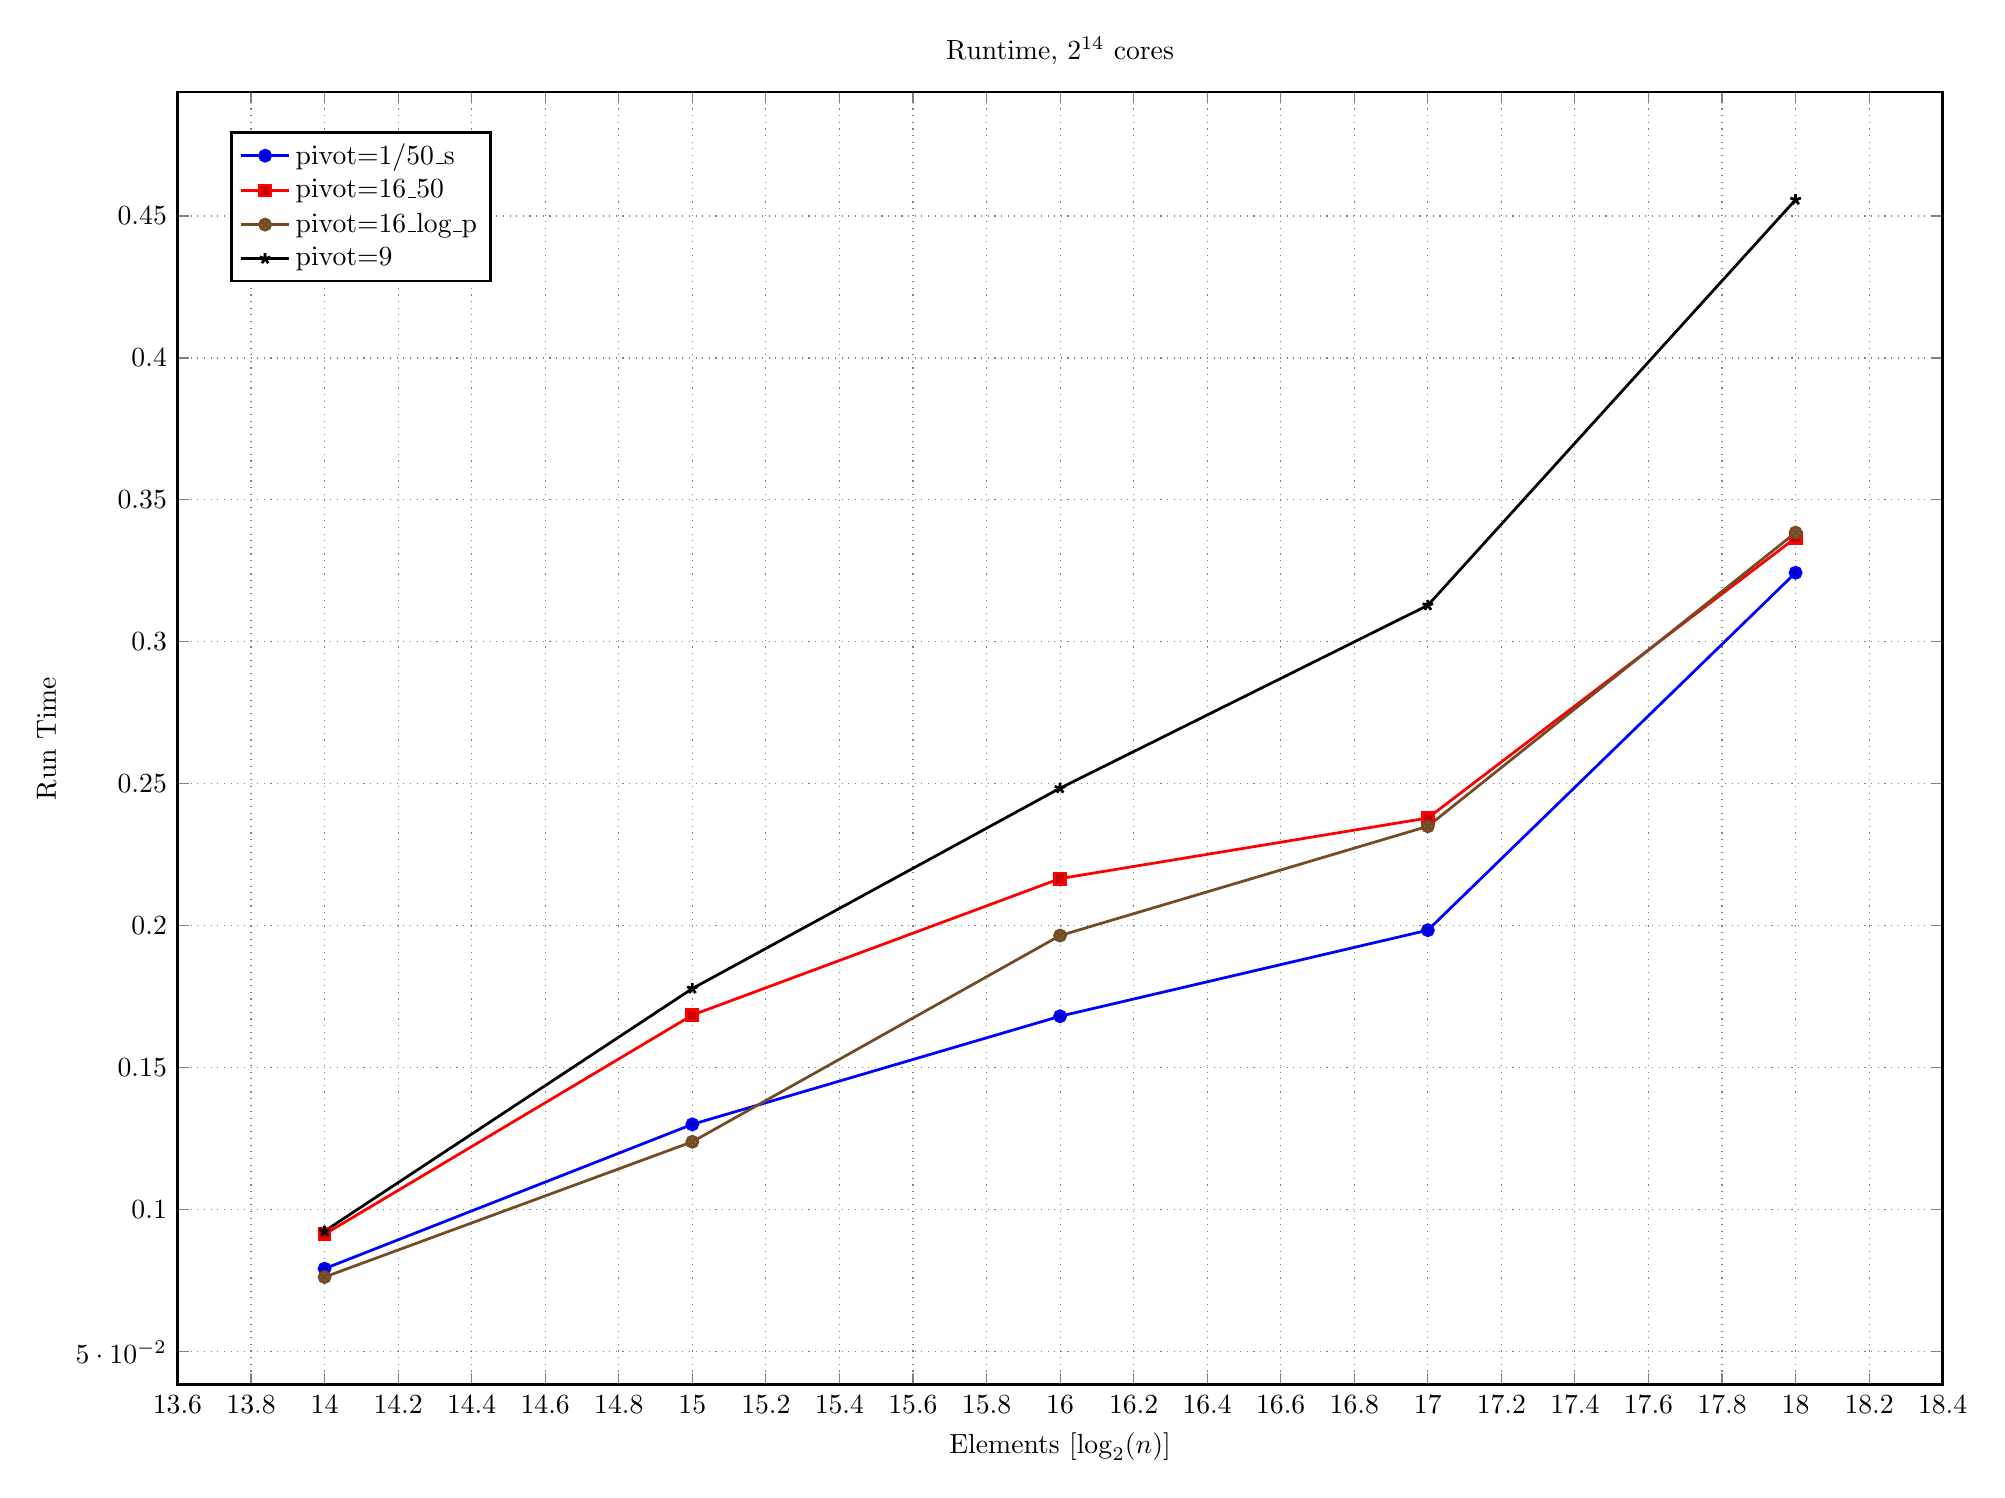
\begin{tikzpicture}
  \begin{axis}[
    title={Runtime, $2^{14}$ cores},
    xlabel={Elements [$\log_2(n)$]},
    ylabel={Run Time},
    ]    

    %% MULTIPLOT(pivot) SELECT LOG(2, elements) AS x, MEDIAN(runtime) AS y, MULTIPLOT
    %% FROM Results 
    %% WHERE size=POWER(2,14) AND x>=14 AND (pivot="9" OR pivot="16_log_p" OR pivot="1/50_s" OR pivot ="16_50")
    %% GROUP BY MULTIPLOT, x  ORDER BY MULTIPLOT, x
    \addplot coordinates { (14.0,0.0792645) (15.0,0.130099) (16.0,0.168172) (17.0,0.198474) (18.0,0.324364) };
    \addlegendentry{pivot=1/50\_s};
    \addplot coordinates { (14.0,0.0914004) (15.0,0.168576) (16.0,0.216647) (17.0,0.237986) (18.0,0.336655) };
    \addlegendentry{pivot=16\_50};
    \addplot coordinates { (14.0,0.0763139) (15.0,0.123955) (16.0,0.196591) (17.0,0.235059) (18.0,0.338498) };
    \addlegendentry{pivot=16\_log\_p};
    \addplot coordinates { (14.0,0.0924869) (15.0,0.177908) (16.0,0.248493) (17.0,0.312887) (18.0,0.455723) };
    \addlegendentry{pivot=9};

  \end{axis}
\end{tikzpicture}
\newpage

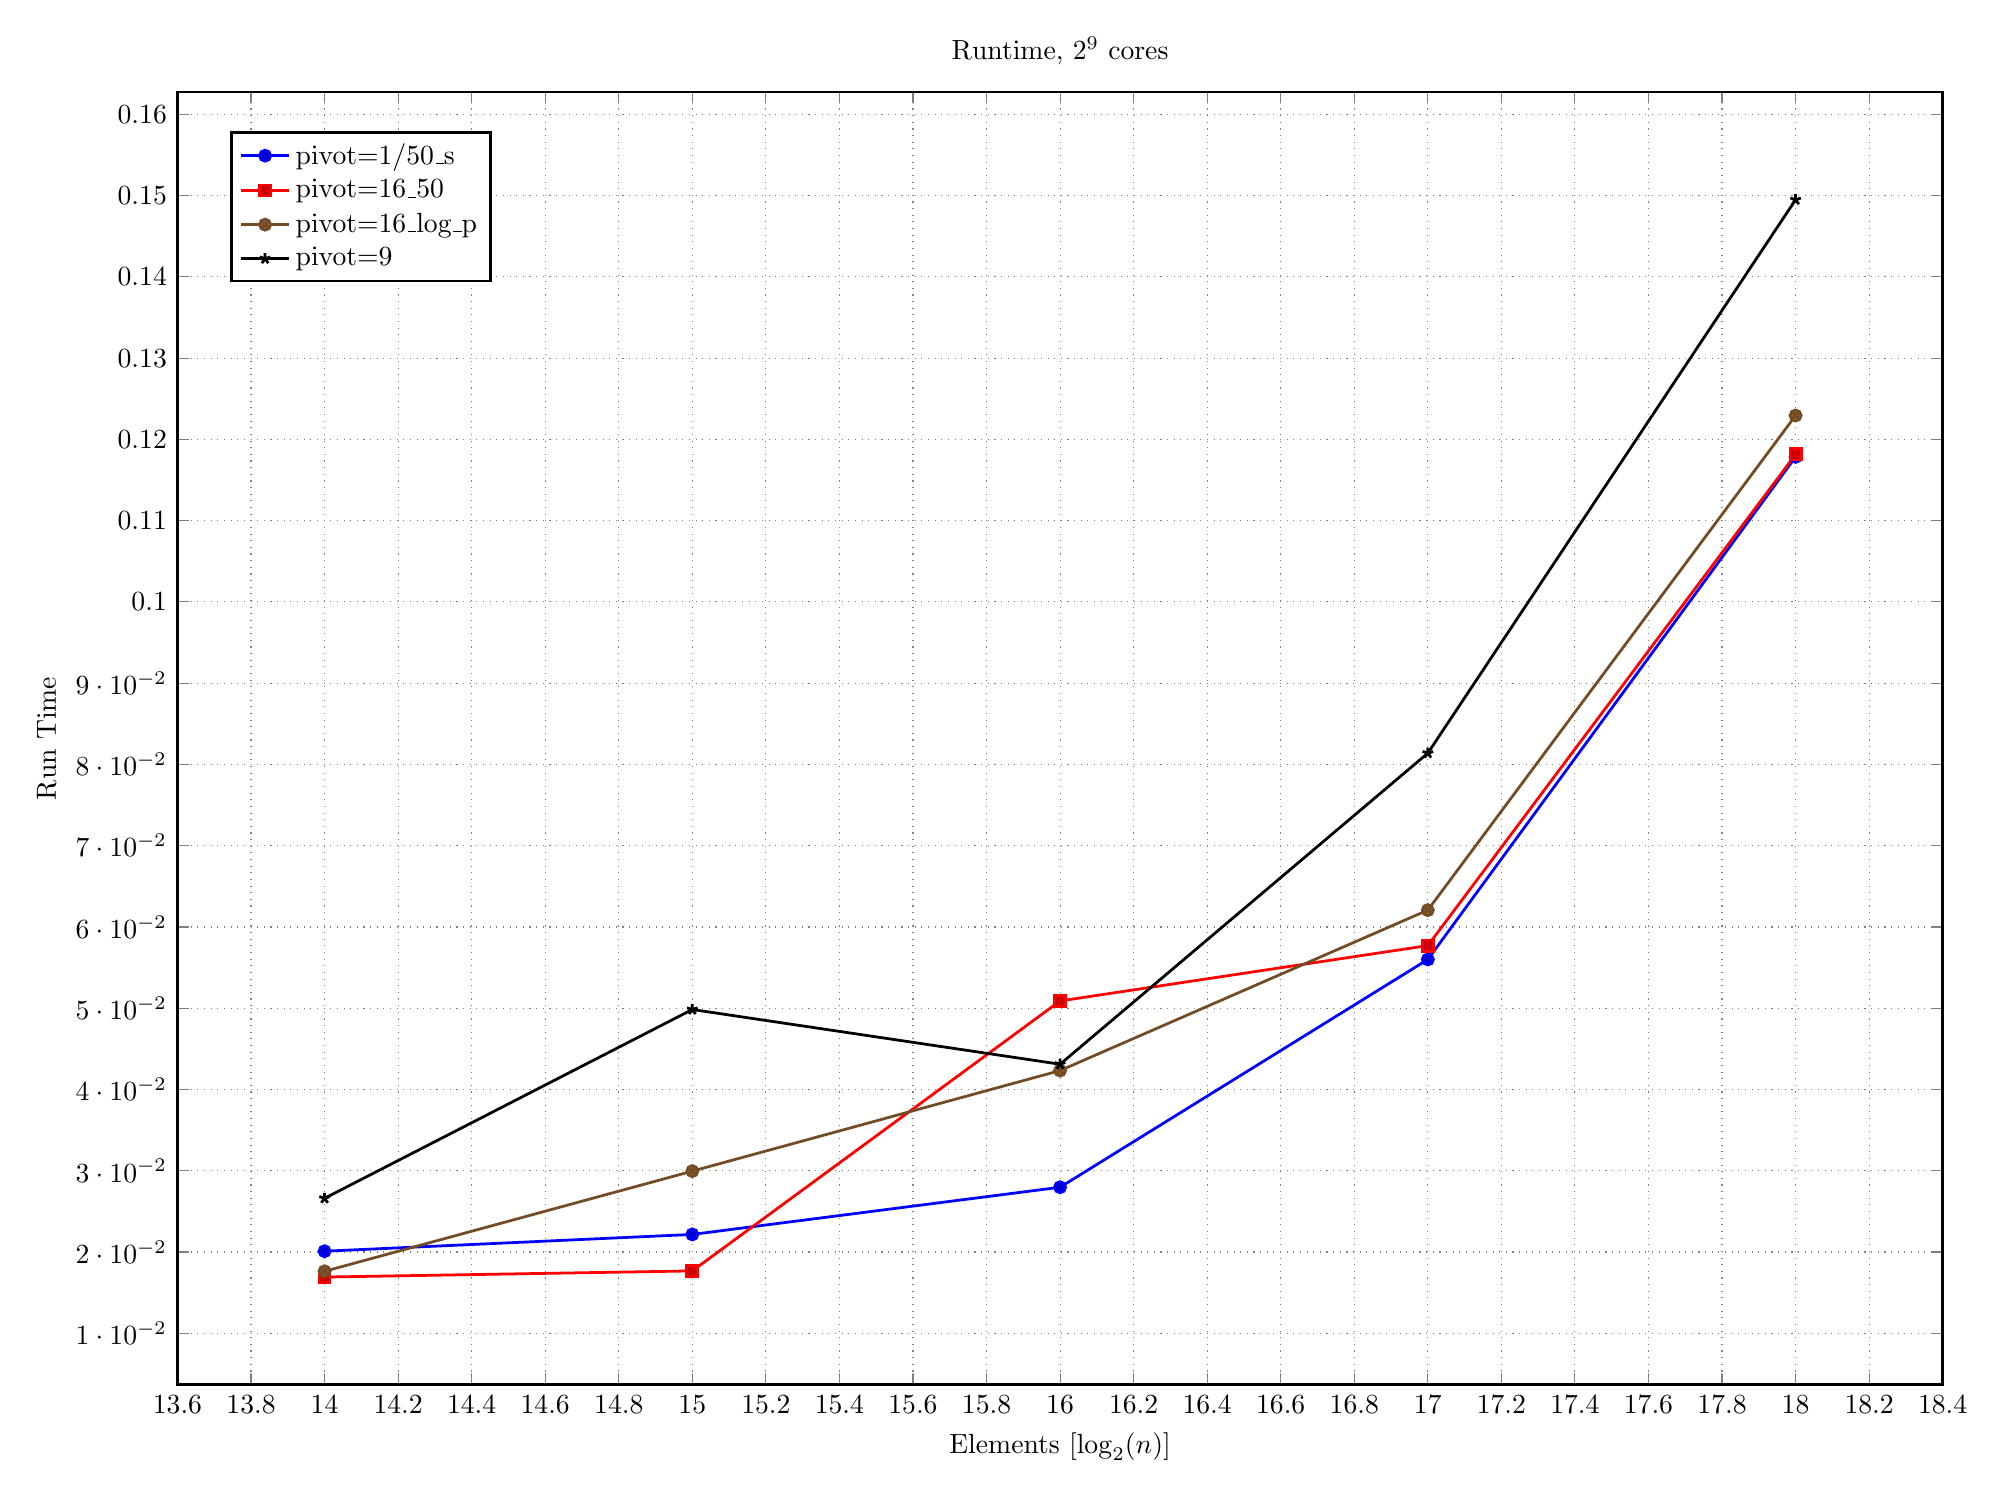
\begin{tikzpicture}
  \begin{axis}[
    title={Runtime, $2^{9}$ cores},
    xlabel={Elements [$\log_2(n)$]},
    ylabel={Run Time},
    ]    

    %% MULTIPLOT(pivot) SELECT LOG(2, elements) AS x, MEDIAN(runtime) AS y, MULTIPLOT
    %% FROM Results 
    %% WHERE size=POWER(2,9) AND x>=14 AND (pivot="9" OR pivot="16_log_p" OR pivot="1/50_s" OR pivot ="16_50")
    %% GROUP BY MULTIPLOT, x  ORDER BY MULTIPLOT, x
    \addplot coordinates { (14.0,0.0201002) (15.0,0.0221652) (16.0,0.0279716) (17.0,0.0559998) (18.0,0.117844) };
    \addlegendentry{pivot=1/50\_s};
    \addplot coordinates { (14.0,0.016919) (15.0,0.0176764) (16.0,0.050895) (17.0,0.0577082) (18.0,0.118147) };
    \addlegendentry{pivot=16\_50};
    \addplot coordinates { (14.0,0.0176281) (15.0,0.0299531) (16.0,0.0423284) (17.0,0.0620737) (18.0,0.122932) };
    \addlegendentry{pivot=16\_log\_p};
    \addplot coordinates { (14.0,0.026611) (15.0,0.0498404) (16.0,0.0431096) (17.0,0.0813853) (18.0,0.149483) };
    \addlegendentry{pivot=9};

  \end{axis}
\end{tikzpicture}
\newpage

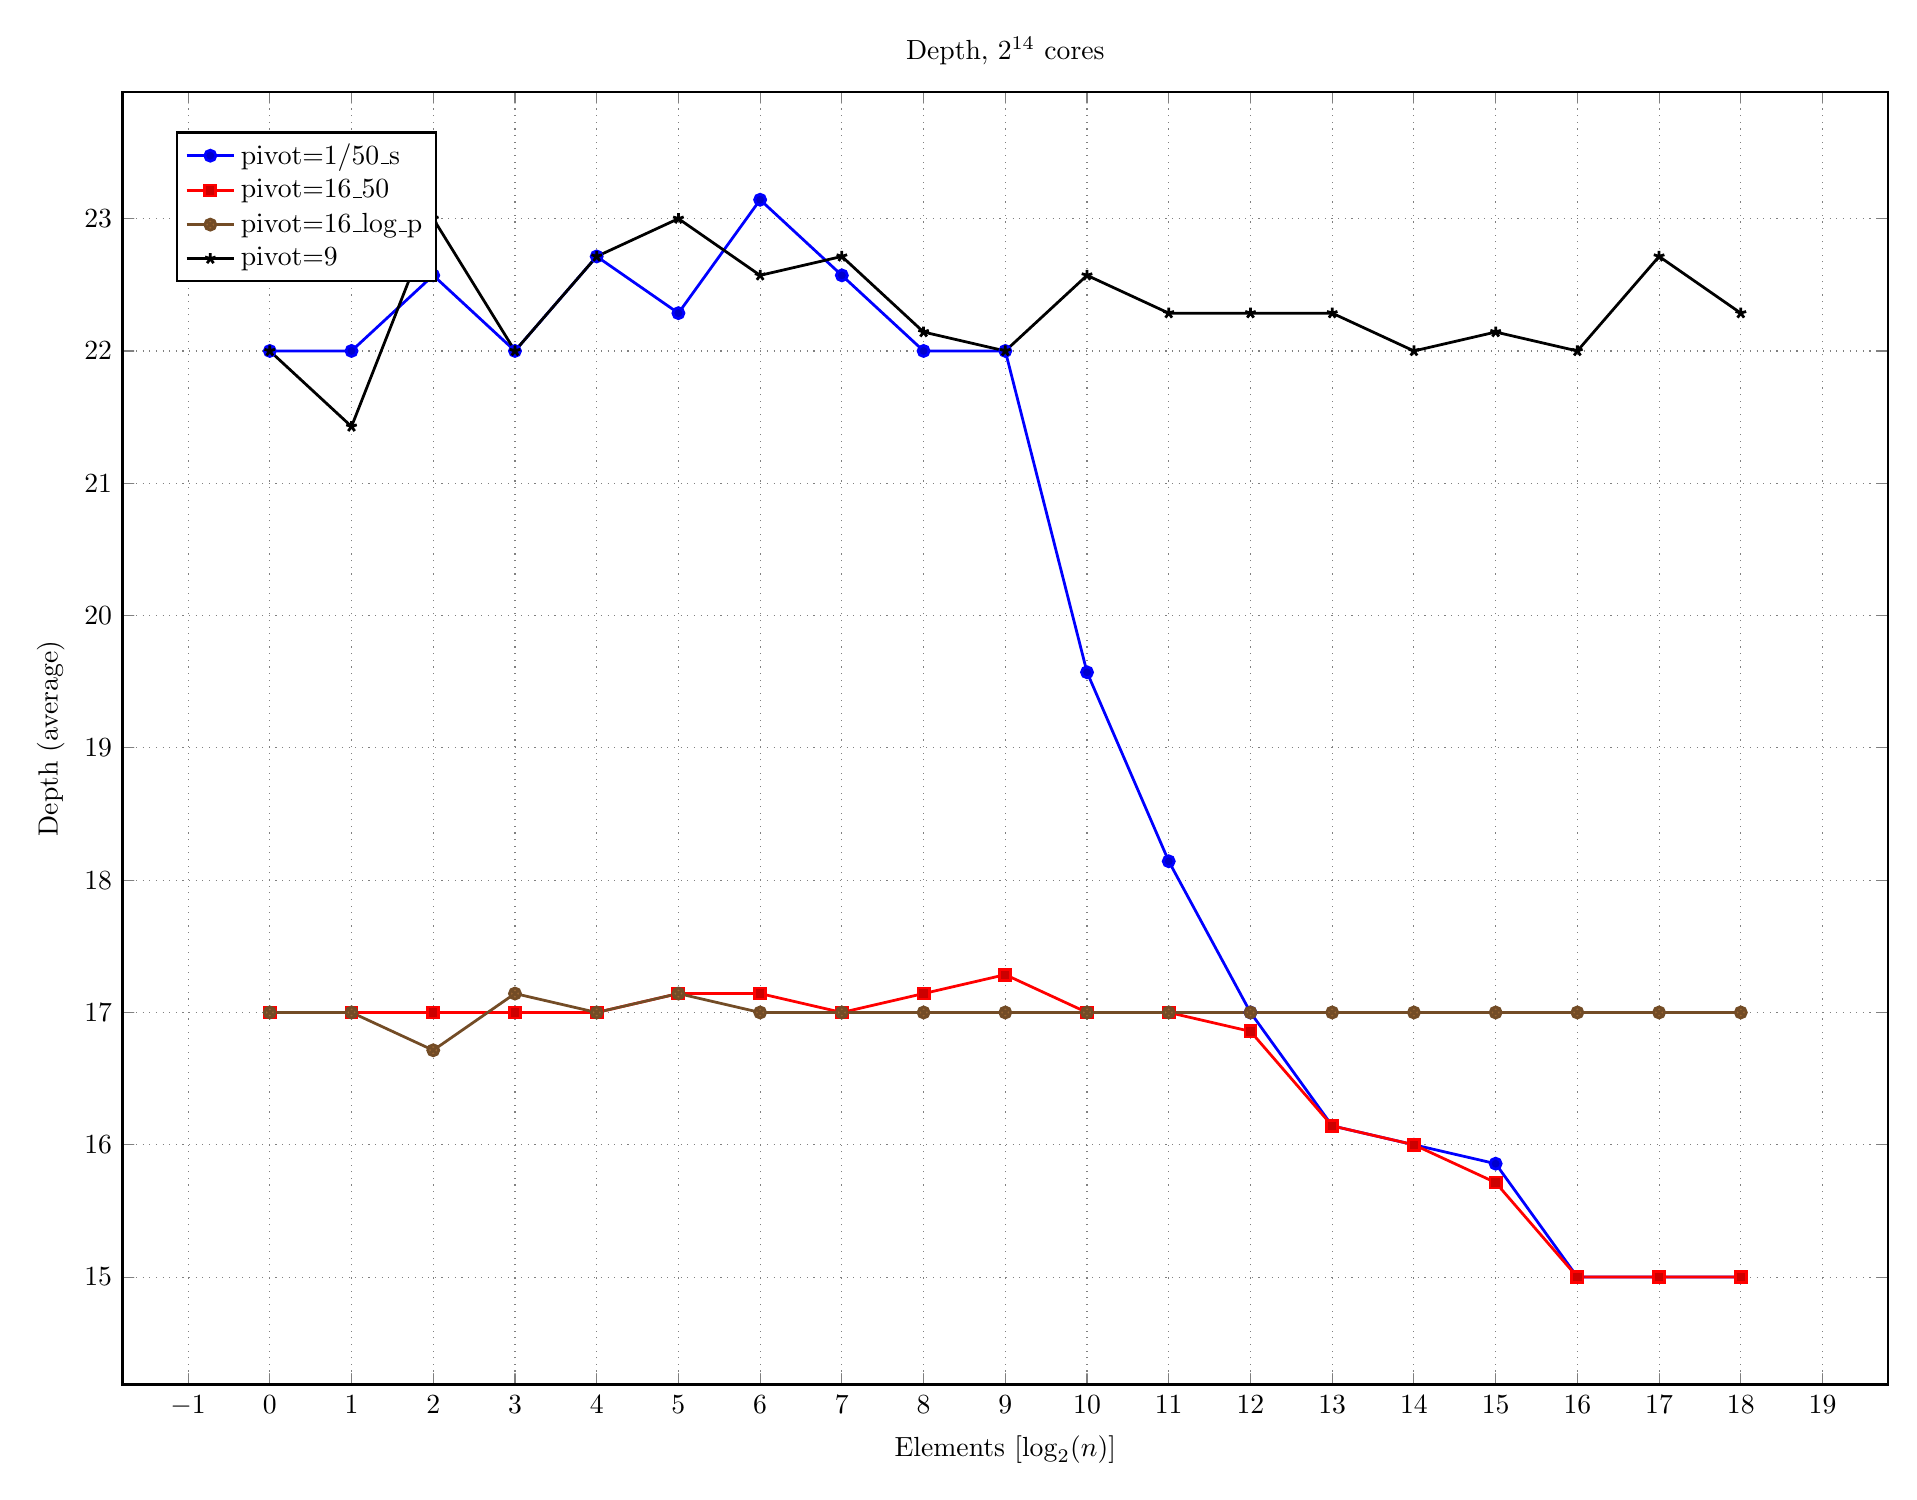
\begin{tikzpicture}
  \begin{axis}[
    title={Depth, $2^{14}$ cores},
    xlabel={Elements [$\log_2(n)$]},
    ylabel={Depth (average)},
    ]    

    %% MULTIPLOT(pivot) SELECT LOG(2, elements) AS x, AVG(depth) AS y, MULTIPLOT
    %% FROM Results 
    %% WHERE size=POWER(2,14) AND (pivot="9" OR pivot="16_log_p" OR pivot="1/50_s" OR pivot ="16_50")
    %% GROUP BY MULTIPLOT, x  ORDER BY MULTIPLOT, x
    \addplot coordinates { (0.0,22.0) (1.0,22.0) (2.0,22.5714) (3.0,22.0) (4.0,22.7143) (5.0,22.2857) (6.0,23.1429) (7.0,22.5714) (8.0,22.0) (9.0,22.0) (10.0,19.5714) (11.0,18.1429) (12.0,17.0) (13.0,16.1429) (14.0,16.0) (15.0,15.8571) (16.0,15.0) (17.0,15.0) (18.0,15.0) };
    \addlegendentry{pivot=1/50\_s};
    \addplot coordinates { (0.0,17.0) (1.0,17.0) (2.0,17.0) (3.0,17.0) (4.0,17.0) (5.0,17.1429) (6.0,17.1429) (7.0,17.0) (8.0,17.1429) (9.0,17.2857) (10.0,17.0) (11.0,17.0) (12.0,16.8571) (13.0,16.1429) (14.0,16.0) (15.0,15.7143) (16.0,15.0) (17.0,15.0) (18.0,15.0) };
    \addlegendentry{pivot=16\_50};
    \addplot coordinates { (0.0,17.0) (1.0,17.0) (2.0,16.7143) (3.0,17.1429) (4.0,17.0) (5.0,17.1429) (6.0,17.0) (7.0,17.0) (8.0,17.0) (9.0,17.0) (10.0,17.0) (11.0,17.0) (12.0,17.0) (13.0,17.0) (14.0,17.0) (15.0,17.0) (16.0,17.0) (17.0,17.0) (18.0,17.0) };
    \addlegendentry{pivot=16\_log\_p};
    \addplot coordinates { (0.0,22.0) (1.0,21.4286) (2.0,23.0) (3.0,22.0) (4.0,22.7143) (5.0,23.0) (6.0,22.5714) (7.0,22.7143) (8.0,22.1429) (9.0,22.0) (10.0,22.5714) (11.0,22.2857) (12.0,22.2857) (13.0,22.2857) (14.0,22.0) (15.0,22.1429) (16.0,22.0) (17.0,22.7143) (18.0,22.2857) };
    \addlegendentry{pivot=9};

  \end{axis}
\end{tikzpicture}
\newpage

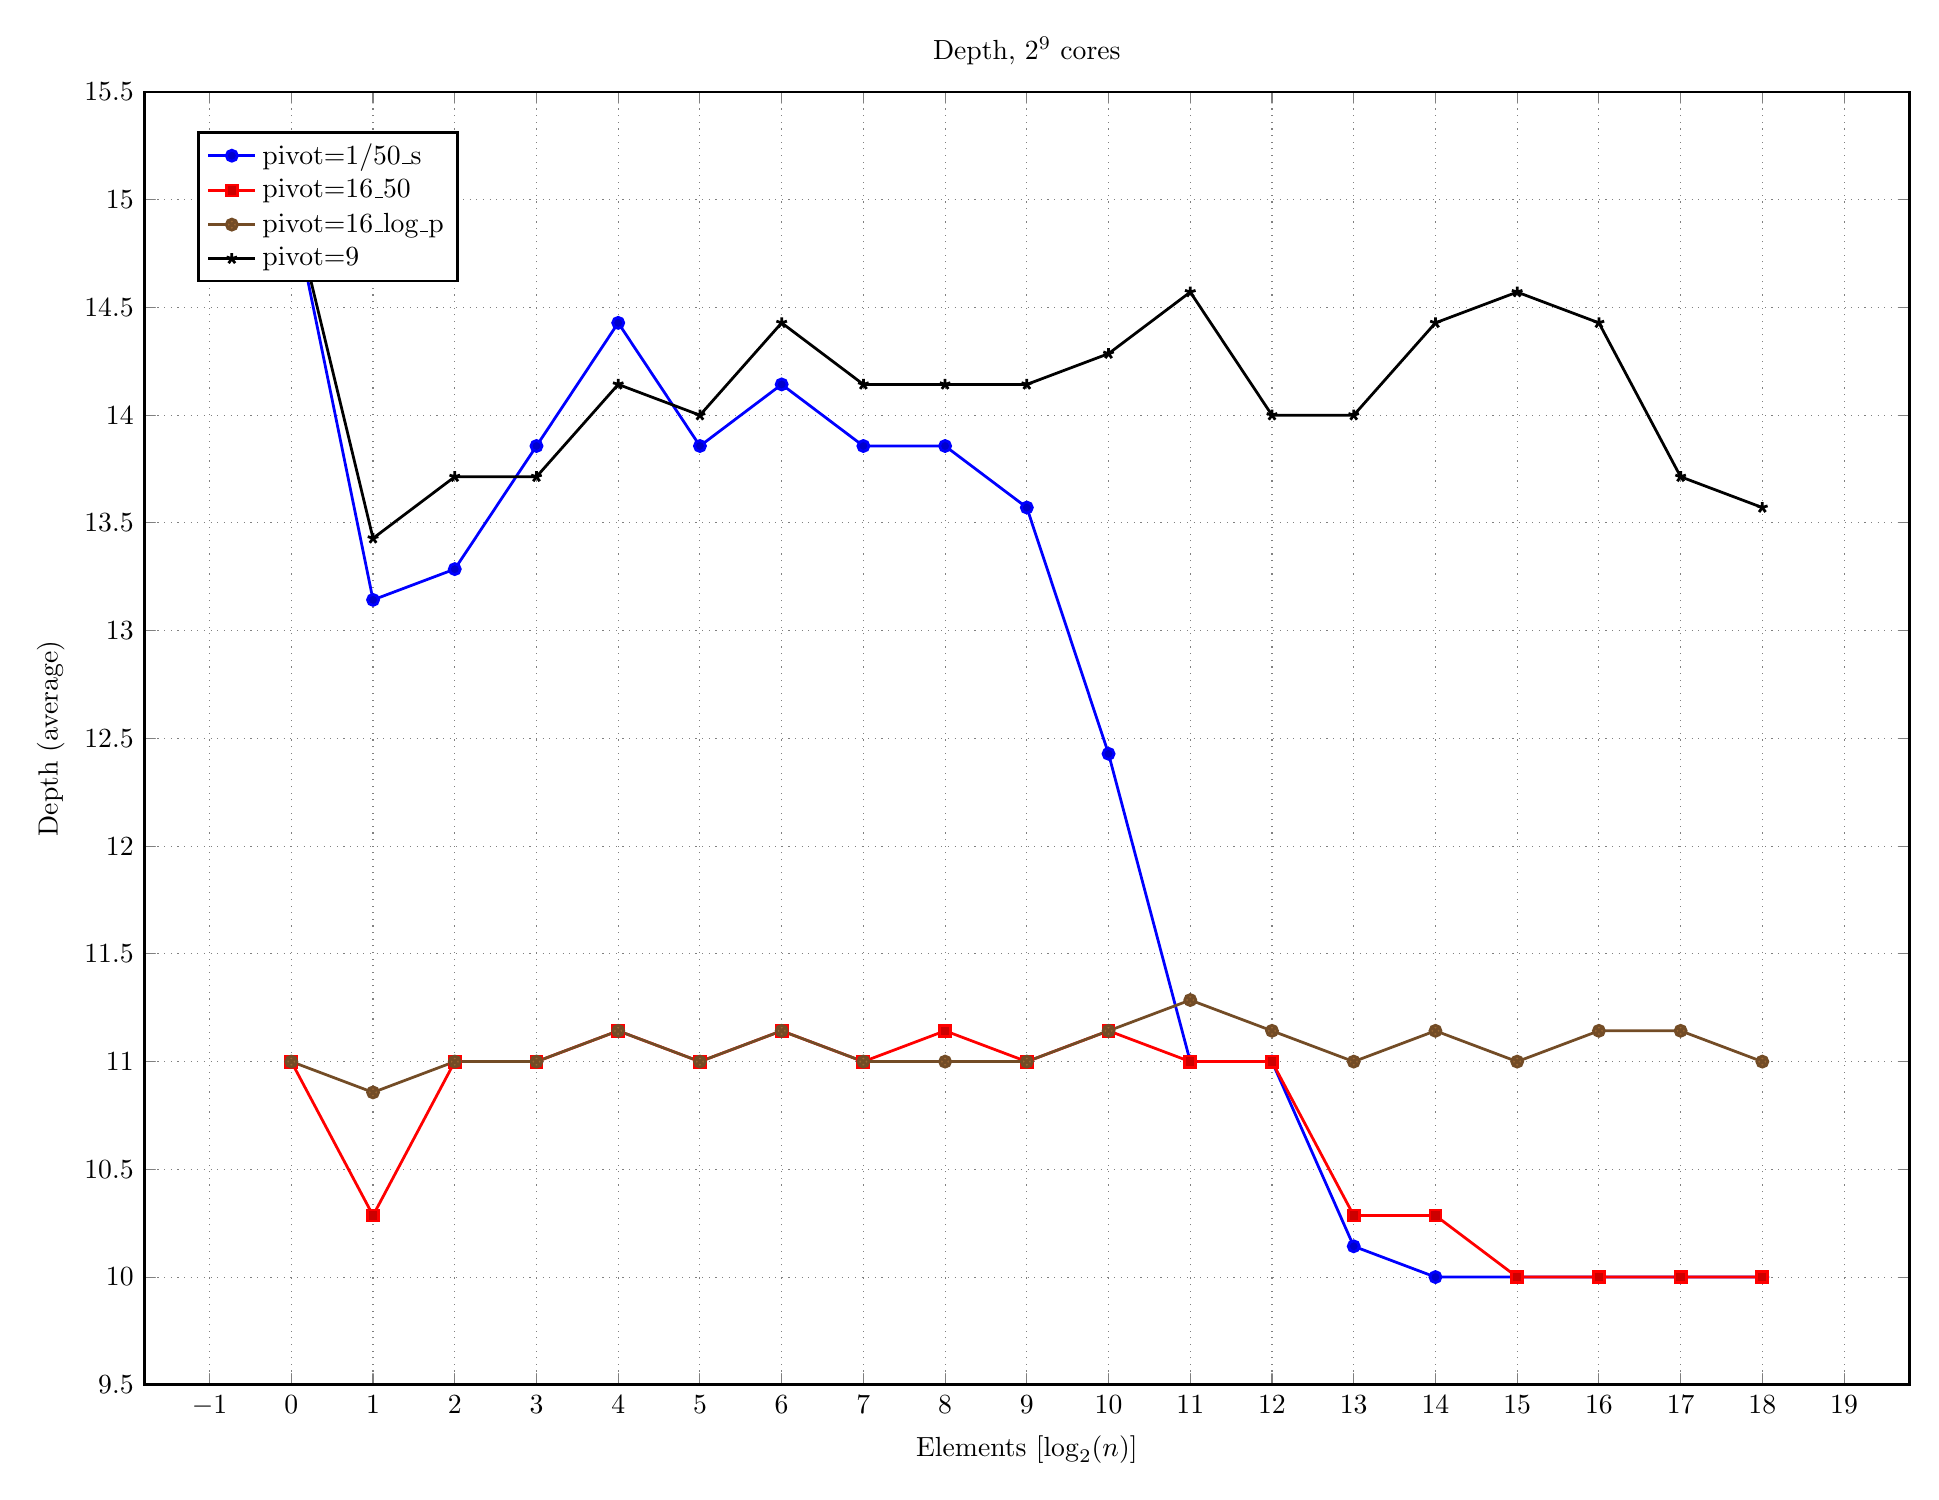
\begin{tikzpicture}
  \begin{axis}[
    title={Depth, $2^{9}$ cores},
    xlabel={Elements [$\log_2(n)$]},
    ylabel={Depth (average)},
    ]    

    %% MULTIPLOT(pivot) SELECT LOG(2, elements) AS x, AVG(depth) AS y, MULTIPLOT
    %% FROM Results 
    %% WHERE size=POWER(2,9) AND (pivot="9" OR pivot="16_log_p" OR pivot="1/50_s" OR pivot ="16_50")
    %% GROUP BY MULTIPLOT, x  ORDER BY MULTIPLOT, x
    \addplot coordinates { (0.0,15.0) (1.0,13.1429) (2.0,13.2857) (3.0,13.8571) (4.0,14.4286) (5.0,13.8571) (6.0,14.1429) (7.0,13.8571) (8.0,13.8571) (9.0,13.5714) (10.0,12.4286) (11.0,11.0) (12.0,11.0) (13.0,10.1429) (14.0,10.0) (15.0,10.0) (16.0,10.0) (17.0,10.0) (18.0,10.0) };
    \addlegendentry{pivot=1/50\_s};
    \addplot coordinates { (0.0,11.0) (1.0,10.2857) (2.0,11.0) (3.0,11.0) (4.0,11.1429) (5.0,11.0) (6.0,11.1429) (7.0,11.0) (8.0,11.1429) (9.0,11.0) (10.0,11.1429) (11.0,11.0) (12.0,11.0) (13.0,10.2857) (14.0,10.2857) (15.0,10.0) (16.0,10.0) (17.0,10.0) (18.0,10.0) };
    \addlegendentry{pivot=16\_50};
    \addplot coordinates { (0.0,11.0) (1.0,10.8571) (2.0,11.0) (3.0,11.0) (4.0,11.1429) (5.0,11.0) (6.0,11.1429) (7.0,11.0) (8.0,11.0) (9.0,11.0) (10.0,11.1429) (11.0,11.2857) (12.0,11.1429) (13.0,11.0) (14.0,11.1429) (15.0,11.0) (16.0,11.1429) (17.0,11.1429) (18.0,11.0) };
    \addlegendentry{pivot=16\_log\_p};
    \addplot coordinates { (0.0,15.0) (1.0,13.4286) (2.0,13.7143) (3.0,13.7143) (4.0,14.1429) (5.0,14.0) (6.0,14.4286) (7.0,14.1429) (8.0,14.1429) (9.0,14.1429) (10.0,14.2857) (11.0,14.5714) (12.0,14.0) (13.0,14.0) (14.0,14.4286) (15.0,14.5714) (16.0,14.4286) (17.0,13.7143) (18.0,13.5714) };
    \addlegendentry{pivot=9};

  \end{axis}
\end{tikzpicture}
\newpage


\end{center}

\end{document}

%%%%%%%%%%%%%%%%%%%%%%%%%%%%%%%%%%%%%%%%%%%%%%%%%%%%%%%%%%%%%%%%%%%%%%%%%%%%%%%%
